%% !TEX root = manual.tex

\section{Fat Tree}
\label{sec:tutorial:fattree}

SST provides a very flexible fat-tree topology which allows both full bandwidth and tapered bandwidth configurations using either uniform or non-uniform switches.
This flexibility requires a farily complicated set of input parameters which are best introduced by examining a couple of example configurations.  Consider the full-bandwidth topology in Figure~\ref{fig:topologies:fullfattree} which uses uniform 8-port switches throughout.

\begin{figure}[h!]
\centering
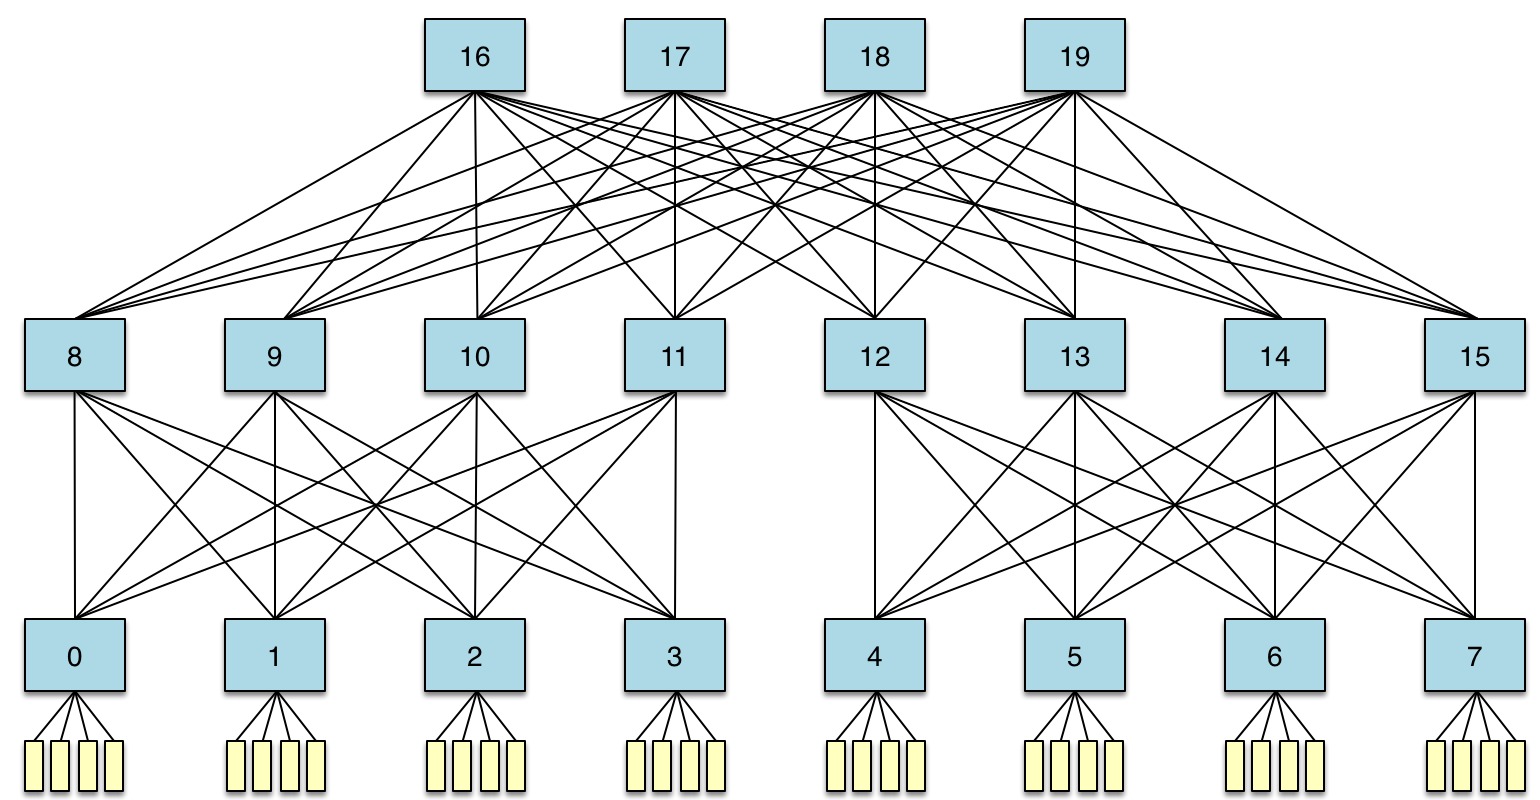
\includegraphics[width=0.7\textwidth]{figures/topologies/fattree4.png}
\caption{Full-bandwidth fat-tree topology using uniform 8-port switches.}
\label{fig:topologies:fullfattree}
\end{figure}

The SST fat-tree is strictly a 3-level topology, with the switch levels refered to as leaf (bottom), aggregation (middle), and core (top).
Interconnected leaf and aggregation switches form an aggregation subtree, which forms the basic unit of a fat-tree topology.
The structure of the aggregation subtree is, itself, flexible and places few constraints on the number of subtrees or the way they are connected to the core level.
In Figure~\ref{fig:topologies:fullfattree}, there are 4 leaf switches and 4 aggregation switches per subtree, and each leaf switch has a concentration of four nodes per switch.
Balancing bandwidth, there are 4 ports going up from each leaf switch and 4 ports going down from each aggregation switch.
This subtree can be specified as follows:

\begin{ViFile}
topology.leaf_switches_per_subtree = 4
topology.agg_switches_per_subtree = 4
topology.concentration = 4
topology.up_ports_per_leaf_switch = 4
topology.down_ports_per_agg_switch = 4
\end{ViFile}

In this example we have 2 aggregation subtrees.
There are four ports going up from each aggregation switch.
All of the ports on the core switches go down, so the number of core switches required (4) is only half the number of total aggregation switches (8).
This core configuration can be specified as follows:

\begin{ViFile}
topologies.num_agg_subtrees = 2
topologies.num_core_switches = 4
topologies.up_ports_per_agg_switch = 4
topologies.down_ports_per_core_switch = 8
\end{ViFile}

Putting it all together with the topology name results in:

\begin{ViFile}
topology.name = fat_tree
logy.leaf_switches_per_subtree = 4
topology.agg_switches_per_subtree = 4
topology.concentration = 4
topology.up_ports_per_leaf_switch = 4
topology.down_ports_per_agg_switch = 4
topologies.num_agg_subtrees = 2
topologies.num_core_switches = 4
topologies.up_ports_per_agg_switch = 4
topologies.down_ports_per_core_switch = 8
\end{ViFile}

The next example, though somewhat contrived, better demonstrates the fat-tree input flexibility.
Suppose that one wanted to use the same 8-port switches to construct a 3-level fat-tree that was both cheaper and had more endpoints (nodes), at the cost of interswitch bandwidth.
One possible configuration is shown in Figure~\ref{fig:topologies:taperedfattree}.

\begin{figure}[h!]
\centering
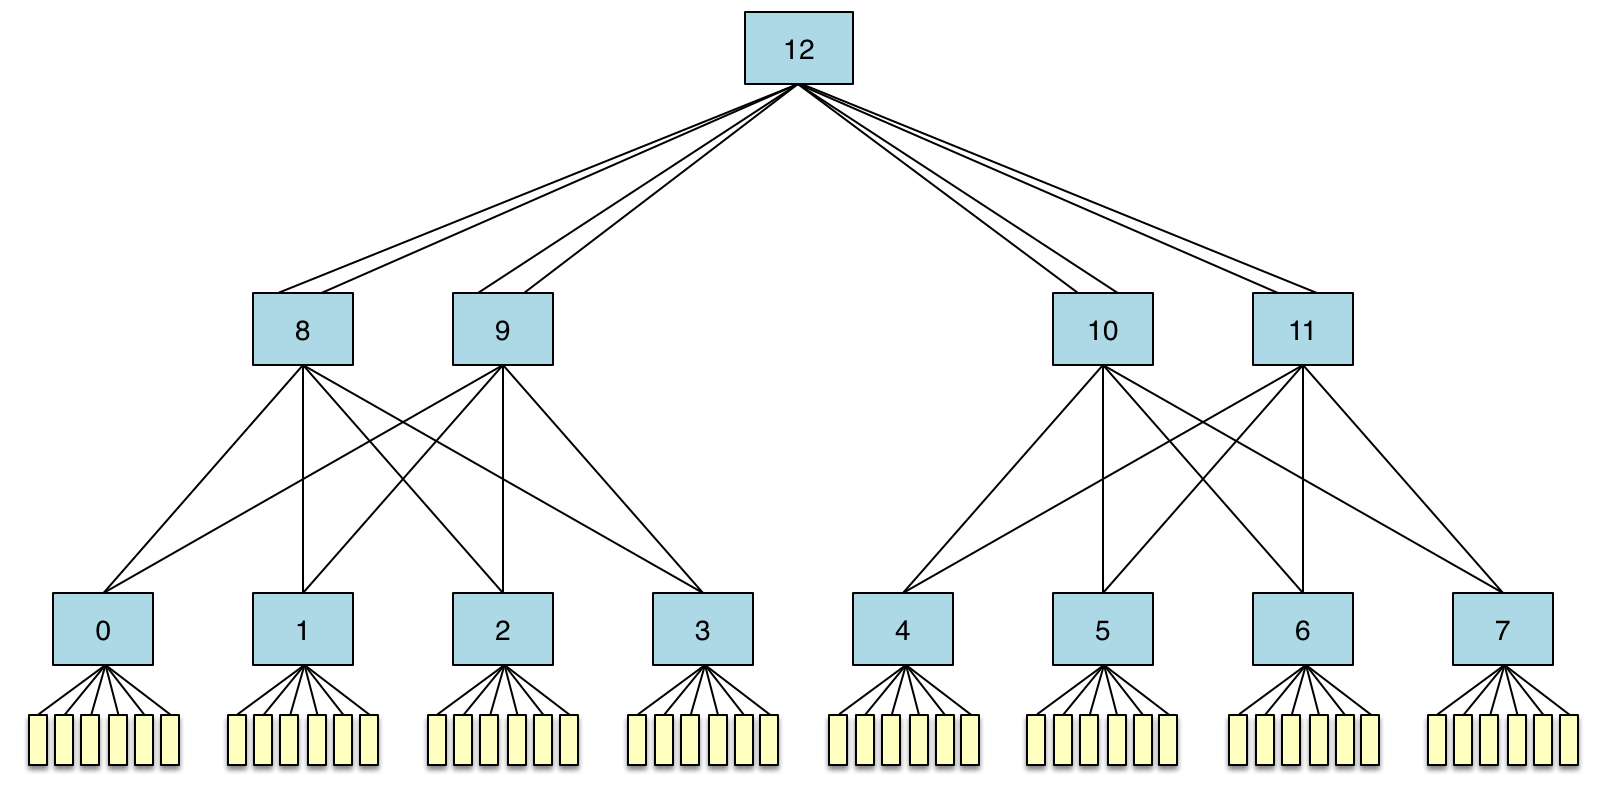
\includegraphics[width=0.7\textwidth]{figures/topologies/fattree4-tapered.png}
\caption{A tapered fat-tree topology using uniform 8-port switches.}
\label{fig:topologies:taperedfattree}
\end{figure}

Here the concentration has been increased to 6 nodes per leaf switch, leaving only two up ports per leaf switch.
Thus an aggregation subtree has a total of only 8 leaf up ports, which requires at least two aggregation switches (in order to have any ports left to connect into the core).
Each aggregation switch is then required to have 4 ports heading down.
The subtree can be configured as follows:

\begin{ViFile}
topology.leaf_switches_per_subtree = 4
topology.agg_switches_per_subtree = 2
topology.concentration = 6
topology.up_ports_per_leaf_switch = 2
topology.down_ports_per_agg_switch = 4
\end{ViFile}

There are a total of four aggregation switches.
If the bandwidth is allowed to taper again, a single 8-port core switch can accomodate 2 ports coming up from each aggregation switch.
This core configuration can be specified as follows:

\begin{ViFile}
topologies.num_agg_subtrees = 2
topologies.num_core_switches = 1
topologies.up_ports_per_agg_switch = 2
topologies.down_ports_per_core_switch = 8
\end{ViFile}

This is a heavily tapered tree and also has the downside of using only 6 ports per switch in the aggregation level.
This example was chosen more for its illustrative rather than practical value, though there are certainly applications where it would be perfectly adequate. 
More practical tapering becomes an option when you increase the number of ports per switch, but visualizations become more difficult to grasp.

The following constraints must be met for a valid configuration.
\begin{itemize}
\renewcommand{\labelitemii}{$\circ$}
\item Down ports must equal up ports: leaf up ports (\inlineshell{leaf_switches_per_subtree} $\cdot$ \inlineshell{up_ports_per_leaf_switch}) must equal aggregation down ports (\inlineshell{agg_switches_per_subtree} $\cdot$ \inlineshell{down_ports_per_agg_switch}), and total aggregation up ports (\inlineshell{up_ports_per_agg_switch} $\cdot$ \inlineshell{agg_switches_per_subtree} $\cdot$ \inlineshell{num_agg_subtrees}) must equal total core down ports (\inlineshell{num_core_switches} $\cdot$ \inlineshell{down_ports_per_core_switch}).
\item Need enough down ports -- each switch must have at least one link into each "unit" (subtree or switch, depending on level) below it:  \inlineshell{down_ports_per_core_switch} must be $\geq$ \inlineshell{num_agg_subtrees}, and \inlineshell{down_ports_per_agg_switch} must be $\geq$ \inlineshell{leaf_switches_per_subtree}.
\item Need enough up ports -- each "unit" (subtree or switch) must have at least one link into each switch above it: \inlineshell{up_ports_per_agg_switch} $\cdot$ \inlineshell{agg_switches_per_subtree} must be $\geq$ \inlineshell{num_core_switches}, and \inlineshell{up_ports_per_leaf_switch} must be $\geq$ \inlineshell{agg_switches_per_subtree}.
\item Connections need to be regular: 1) \inlineshell{down_ports_per_core_switch} $\bmod$ \inlineshell{num_agg_subtrees} must equal zero, 2) \inlineshell{down_ports_per_agg_switch} $\bmod$ \inlineshell{leaf_switches_per_subtree} must equal zero, 3) \inlineshell{up_ports_per_leaf_switch} $\bmod$ \inlineshell{agg_switches_per_subtree} must equal zero
\end{itemize}

\subsection{Switch Crossbar Bandwidth Scaling}
\label{subsec:fattree:xbarbw}

Allowing non-uniform switches in the topology implies that switch crossbar bandwidth should be non-uniform as well.
By default, SST assumes \inlineshell{switch.xbar.bandwidth} specifies the bandwidth for the switch type with the lowest port count.
The crossbar bandwidth is scaled by the total number of ports for all other switch types. 
Input keywords are provided to override this default behavior.
For the tapered-bandwidth example above, uniform switch bandwidth can be maintained by setting all bandwidth scaling to 1.0:

\begin{ViFile}
topology.leaf_bandwidth_multiplier = 1.0
topology.agg_bandwidth_multiplier = 1.0
topology.core_bandwidth_multiplier = 1.0
\end{ViFile}

\subsection{Routing}
\label{subsec:fattree:routing}

The fat-tree topology should be used in conjunction with \inlineshell{router = fat_tree}, which will maximize the utilization of path diversity.
There is a \inlineshell{fat_tree_minimal} router which will use the lowest numbered valid port for any destination; this will result in poor network performance and is primarily useful for testing and perhaps experiments where network contention is desired.
